\documentclass{seminar}
%\documentclass[german]{seminar}

\usepackage{tikz}
\usepackage{booktabs}
\usepackage{multirow}
\usetikzlibrary{shapes,arrows}

\newcommand{\q}[1]{``#1''}
\newcommand{\tabitem}{~~\llap{\textbullet}~~}
\newcommand{\exampleQuote}[1]{\small{\textit{``#1''}}}
\newcommand{\obsrvQuote}[1]{\textit{``#1''} }
\newcommand{\red}[1]{{\color{red}#1}}
\hyphenation{PICOT}
\hyphenation{FINER}
\hyphenation{EBSE}

\begin{document}

\semcover{A structured approach to Evidence-based software engineering in empirical software engineering research.}
	{M. Danz, T. Gr\"af, C. Michel}
	{student@student.kit.edu}
	{Andrei Miclaus}
	{miclaus@teco.edu}


% TODO sort the sections

% !TEX root = ../../seminar.tex

\begin{abstract}
~\\\\\textbf{Background}: It was found, that some students struggle with scientific working.\\
\textbf{Objective}: Create a supporting document tailored for students. With a main focus on ease of use and with EBSE in mind to establish it further.\\
\textbf{Results}: Based on literature and experience, a process and supporting documents are created. The process is based on EBSE. To make the document easy to use, it incorporates simple and clear design as well as concise instructions.\\
\textbf{Limitations}: This work is mainly aimed at computer science students and needs to be evaluated in future work.

\semkeywords{
software engineering, 
evidence-based software engineering,
EBSE,
scientific working,
flowchart,
checklist,
student workflow}

\end{abstract}

% !TEX root = ../../seminar.tex


\section{Introduction}
\label{sec:introduction}

It was observed\todosoft{rephrase} that most software build in a bachelor's or master's thesis is poorly evaluated or not evaluated at all. Therefore our initial aim was finding or creating a method to evaluate and compare software suited for students.

But we soon discovered a major problem: Large pieces of software are hard to evaluate because effects can be hard to isolate.
To find out which software \todosoft{SW architecture, devel method..} is more suitable for a given problem, measurements are needed for a quantitative comparison. Moreover, a controlled study is needed to attain valid measurements that allow comparison. Students often struggle with obtaining this \emph{empirical evidence} (see table \ref{table:issuesEBSE}) leading to unusable results making a proper comparison difficult or not possible at all. 

So we revised the question to: How to create a supporting system for students helping to improve the quality (in particular the substantiality) of their studies in the domain of software engineering.

The final system we intend is an electronical\todosoft{digital? should this be here or just in dicussion because it is not actually part of this paper.} database containing a collection of experiments. The system is meant to simplify searching, scanning and comparison of experiments. Allowing to quickly find existing evidence that can be used for software design decisions. To populate that collection, a process to create evidence correctly and a compact representation of the results are needed. We propose two documents: \emph{\checklist} to guide students through the scientific process and \emph{\briefingform} for a compact, structured and complete resume of the conducted experiment. 


\todo{rest of chapter are notes:}
\begin{itemize}
\item experimentation/empiricism in CS?
\item \q{should computer scientists experiment more?, Tichy 1997}
\item Experimental evaluation in CS: A quantitative study, 1994: 40\% of papers requiring quant evaluation have none (other disciplins: 15\%)
\item \q{A survey of Controlled Experiments in SE, 2005} from 1993 to 2002: 1,9\% of software engineering paper report controlled experiments
\item \q{Belief \& Evidence in Empirical Software Engineering}, 2016: programmers have strong beliefs, primarily formed by personal opinion (research papers just above "other", below peer opinion, mentor opinion and trade journals); beliefs vary between projects, but do not necessarily correspond with evidence in that project
\item \q{Incorrect results in software engineering experiments: How to improve research practices}, 2016: research and publication bias quite common, need to improve research practices (a key: avoid experiments with low statistical power)
\end{itemize}


In section \ref{sec:related work} \emph{evidence-based software engineering} (EBSE) and structured abstracts are introduced. EBSE is the foundation of the process introduced later in section \ref{sec:research process}. Therefore, the idea behind EBSE is very fundamental  for this paper.\\
Structured abstracts are used as a base for the form introduced in section \ref{sec:briefing form}.\\
















	\section{Fundamental Principles}

short introduction to EBSE,..

\begin{itemize}
	\item \textbf{Evidence-based approach}: integrate all available research (evidence) in decision making process
	\item \textbf{Aim}: \q{EBSE aims to improve decision making related to software development and maintenance by integrating current best evidence from research with practical experience and human values.} \cite{EBSEpract}
	\item \textbf{Five steps} of practising EBSE \cite{EBSE}:
		\begin{enumerate}
			\item Ask an answerable question.
			\item Find the best evidence that answers that question.
			\item Critically appraise this evidence.
			\item Apply the evidence (and critical appraisal).
			\item Evaluate the performance in previous steps.
		\end{enumerate}
		$\rightarrow$ important tool: Systematic Literature Review (SLR)
	\item \textbf{SLR} \cite{keele2007}: identify and interpret all available literature regarding a research question
		$\rightarrow$ papers should be written for synthesis (TODO requirements for this, common mistakes/problems?)
\end{itemize}
	\section{Related Work}
SEED, "a preliminary empirical investigation of the use of EBSE by under-graduate students"


\section{Knowledge Management}
TODO \newline
	\subsection{Formulating Research Question and Hypothesis}

For researchers to produce relevant results and understand their research domain fully, the step of developing a good research question, with a supporting hypothesis and sometimes objectives is integral \cite{Farrugia2009}. These components should be carefully designed \emph{before} conducting the study that tries to answer the question. Otherwise it is more likely to produce questions that are already answered, or \obsrvQuote{could potentially lead to spuriously positive findings of association through chance alone.} \cite[p. 280]{Farrugia2009} 

		\subsubsection{Research Question}

The question the later study is designed to answer is called research question \cite{Vickers}. It should be an answerable question and address a relevant issue in the research area \cite{Dyba2005}. Preceding a research question is the need for a deep understanding of the topics that have already been studied, in order to produce questions which drive knowledge further. The questions that arise during the acquisition of knowledge, and cannot be answered by means of EBSE, are likely appropriate questions for further research \cite{Farrugia2009}. \newline
There are two general classes of research questions: qualitative and quantitative questions. Qualitative research states questions which report, describe, or explore a subject \cite[p. 139-141]{Creswell2014}. In computer science as the research field matures these questions become more and more rare {\color{red} (find source)}. Therefore focus is on quantitative research questions in this paper. \obsrvQuote{Quantitative research questions inquire about the relationships among variables} \cite[p. 143]{Creswell2014}, and from them emerge quantitative hypotheses. \newline
To understand the structure of research questions Shaw provides a model where she categorizes research questions from software engineering papers in five types \cite{Shaw2002} {\color{red} (maybe cut out)}. \newline
To design a good research question Haynes coined the acronym PICO: Population, Intervention, Comparison group, and Outcome \cite{BrianHaynes2006}. Sometimes Time is added as fifth component, when it is important over what time frame the study is conducted, see Table \ref{table:PICOT}. A research question structured with the PICOT approach supports in restricting the research question and steers thereby hypotheses and study. By restricting the research question researchers can limit bias and increase the internal validity of the study, but a too narrow question may also lead to decreased external validity \cite{Farrugia2009}. \\
Before PICOT Sackett and colleagues suggested that good research questions consist out of three components: Intervention, Context and Outcome \cite{Sackett2000}, which is a more coarse grained decomposition than PICOT. Dyb{\aa} \emph{et al.} displayed a fitting example for this template in software engineering: \obsrvQuote{Does pair programming lead to improved code quality when practiced by professional software developers?} \cite[p. 60]{Dyba2005} Here the intervention is pair programming, the context of interest are professional software developers, and the outcome is improved code quality \cite{Dyba2005}. To verify the quality of a freshly designed research question Hulley \emph{et al.} suggest the use of the FINER criteria. It highlights key aspects of the question and provides thereby new angles to view the proposed study from. The FINER criteria consists of: Feasible, Interesting, Novel, Ethical, and Relevant \cite{Farrugia2009}. A more detailed view of the FINER criteria can be seen in Table \ref{table:FINER}. {\color{red}(TODO specify more tips for writing a good question. Creswell2014)}  


\begin{table}[]
	\centering
	\fbox{
		\begin{tabular}{ p{3em} p{6.5em} p{22em} }
			\textbf{P}	& Population & What specific population are you interested in? \vspace{1em}\\
			
			\textbf{I}	& Intervention (technology) & What is the investigational technology/ intervention? \vspace{1em}\\
			
			\textbf{C}	& Comparison group & What is the main alternative/baseline to compare with the intervention \vspace{1em}\\ 
			
			\textbf{O}	& Outcome & What do you intend to accomplish, measure, improve or affect? \vspace{1em}\\ 
			
			\textbf{T}	& Time & What is the appropriate follow-up time to assess outcome? 
		\end{tabular}	
	}
	\vspace{1em}
	\caption{PICOT criteria adjusted to fit better in computer science research.}
	\label{table:PICOT}
\end{table}

\begin{table}[]
	\centering
	\fbox{
		\begin{tabular}{ p{3em} p{6em} p{22em} }
				\textbf{F}	& Feasible & \tabitem Adequate number of subjects \\
				\multicolumn{2}{l}{} & \tabitem Adequate technical expertise \\
				\multicolumn{2}{l}{} & \tabitem Affordable in time and money \\
				\multicolumn{2}{l}{} & \tabitem Manageable in scope \vspace{1em}\\
				\textbf{I}	& Interesting & \tabitem Getting the answer intrigues investigator, peers and community \vspace{1em}\\
	
				\textbf{N}	& Novel & \tabitem Confirms, refutes or extends previous findings \vspace{1em}\\
	
				\textbf{E}	& Ethical & \tabitem Amendable to a study that institutional review board will approve \vspace{1em}\\ 
				\textbf{R}	& Relevant & \tabitem To scientific knowledge \\
				\multicolumn{2}{l}{} & \tabitem To clinical and health policy \\
				\multicolumn{2}{l}{} & \tabitem To future research
		\end{tabular}	
	}
	\vspace{1em}
	\caption{FINER criteria for a good research question \cite{Farrugia2009}}
	\label{table:FINER}
\end{table}




		\subsubsection{Hypothesis}

\begin{itemize}
	\item What is it?
	\item For what is it?
	\item is testable statement  {\color{red} (find source)}
	\item Only in Quantitative research  {\color{red} (Creswell)}
	\item two-sided/one-sided hypothesis -> use only two-sided  {\color{red} (Farrugia et al.)}
	\item Null hypothesis in empirical work  {\color{red} (Farrugia et al.)}
	\item contains varaibales/population/relationship  {\color{red} (health website)}
	\item How to hypothesis:
	\begin{itemize}
		\item  {\color{red} (Prasad)}
		\item from websites  {\color{red} (find sources)}
		\item  {\color{red} (Creswell)}
	\end{itemize}
\end{itemize}
		\subsubsection{Objectives}

 Sometimes researchers define objectives to their hypotheses. They are active statements that \obsrvQuote{define specific aims of the study and should be clearly stated} \cite[p. 280]{Farrugia2009} at the beginning of research. Objectives help to define the study (e.g. helping to calculate sample size). \cite{Farrugia2009,Vickers} Although we do not include objectives in our \briefingform we would like to mention them for reasons of completeness.
	% !TEX root = ../../seminar.tex

\subsection{Designing, Conducting And Interpreting Experiment}
\label{subsec:designing conducting and interpreting experiment}
To generate evidence, experiments are conducted. To keep the complexity of the study manageable and prevent side effects, it is recommended to answer only one question per experiment. If the question is too extensive for a single experiment, split up the question in sub-questions and recursively start this process with each sub-question.\\
For guidance and documentation through the experiment use \briefingform introduced in section \ref{sec:briefing form}. Since experimenting is a very complex topic and can not be fully covered in this paper, see \cite{Wohlin2012,Tullis2013} for further reading.
	\subsubsection{Conclusion}

\begin{itemize}
	\item is interpretation of experiment results
	\item verification or rejection of $H_0$ and acceptance of $H_1$
	\item Scope of generalization.
\end{itemize}
	\subsection{Structured Abstract}

\begin{itemize}
\item importance: Abstracts, together with the title, are used to identify relevant research, not only in SLRs. Often the abstract is the only part of the paper that can be accessed for free. Therefore abstract and title should contain all necessary information to decide whether a paper (in case of SLR: primary study) is relevant in this context. (TODO source: \q{Procedures for Undertaking Systematic Reviews})
	$\rightarrow$ quality of abstract crucial for research, how to support researcher in writing useful abstracts? Structured Abstracts provide guidance for writer and reader. 
\item Suggestion of elements proposed by Jedlitschka et al.\cite{Jedlitschka2008}: 
	\begin{enumerate}
		\item Background or Context: motivation for conducting the study, previous research
		\item Objective or Aim: Object that is studied, focus and perspective of the study, hypothesis
		\item Method: e.g. experimental design, participants and selection criteria, measurement and analyzing technique...
		\item Results: most important findings (treatment outcome), no interpretation!
		\item Limitations: scope of study, limits of generalization (often as part of conclusion)
		\item Conclusion: Interpretation of results, put results in context
	\end{enumerate}
	(short and early version:\cite{Jedlitschka2005})
	\newline
	Elements similar to \q{IMRAD}-structure (see paper \q{Adoption of structured abstracts by general medical journals and format for a structured abstract})
\item About completeness and clarity of structured abstracts:
	\begin{enumerate}
	\item Structured abstracts include more relevant information and are easier to read than conventional abstracts. \cite{Budgen2008} \cite{Budgen2007}
	\item Inexperienced authors are likely to produce clearer and more complete abstracts when using a structured form.\cite{Budgen2011} 
	\item On average structured abstracts are longer and have better readability than unstructured abstracts. \cite{KBO2008}
	\item these findings are in accordance with the ones in other disciplines (\red{which?, source})
	\end{enumerate}
\item guidelines for construcing structured abstract (from unstructered ones) in \cite{KBO2008}
\item Guide with examples (psychology): \q{how to write a good abstract for scientigic paper.}, C. Andrade
	\newline
	ANSI/NISO Z39.14.1997 (R2015) Guidelines for Abstracts
\item use standard terminology (commonly used industry terms) \cite{Jedlitschka2008}
\item structured abstracts are longer and often size is limited (journals): prioritize traditional elements, still structured: background (one sentence), objective, method, results, and conclusion \cite{Jedlitschka2008}
\end{itemize}


% !TEX root = ../../seminar.tex

\section{Student Process Improvement Document - \checklist}
\label{sec:research process}

\begin{minipage}{\linewidth}
\begin{wrapfigure}{R}{0.3\textwidth}
	\centering
	\vspace{-1.0cm}
	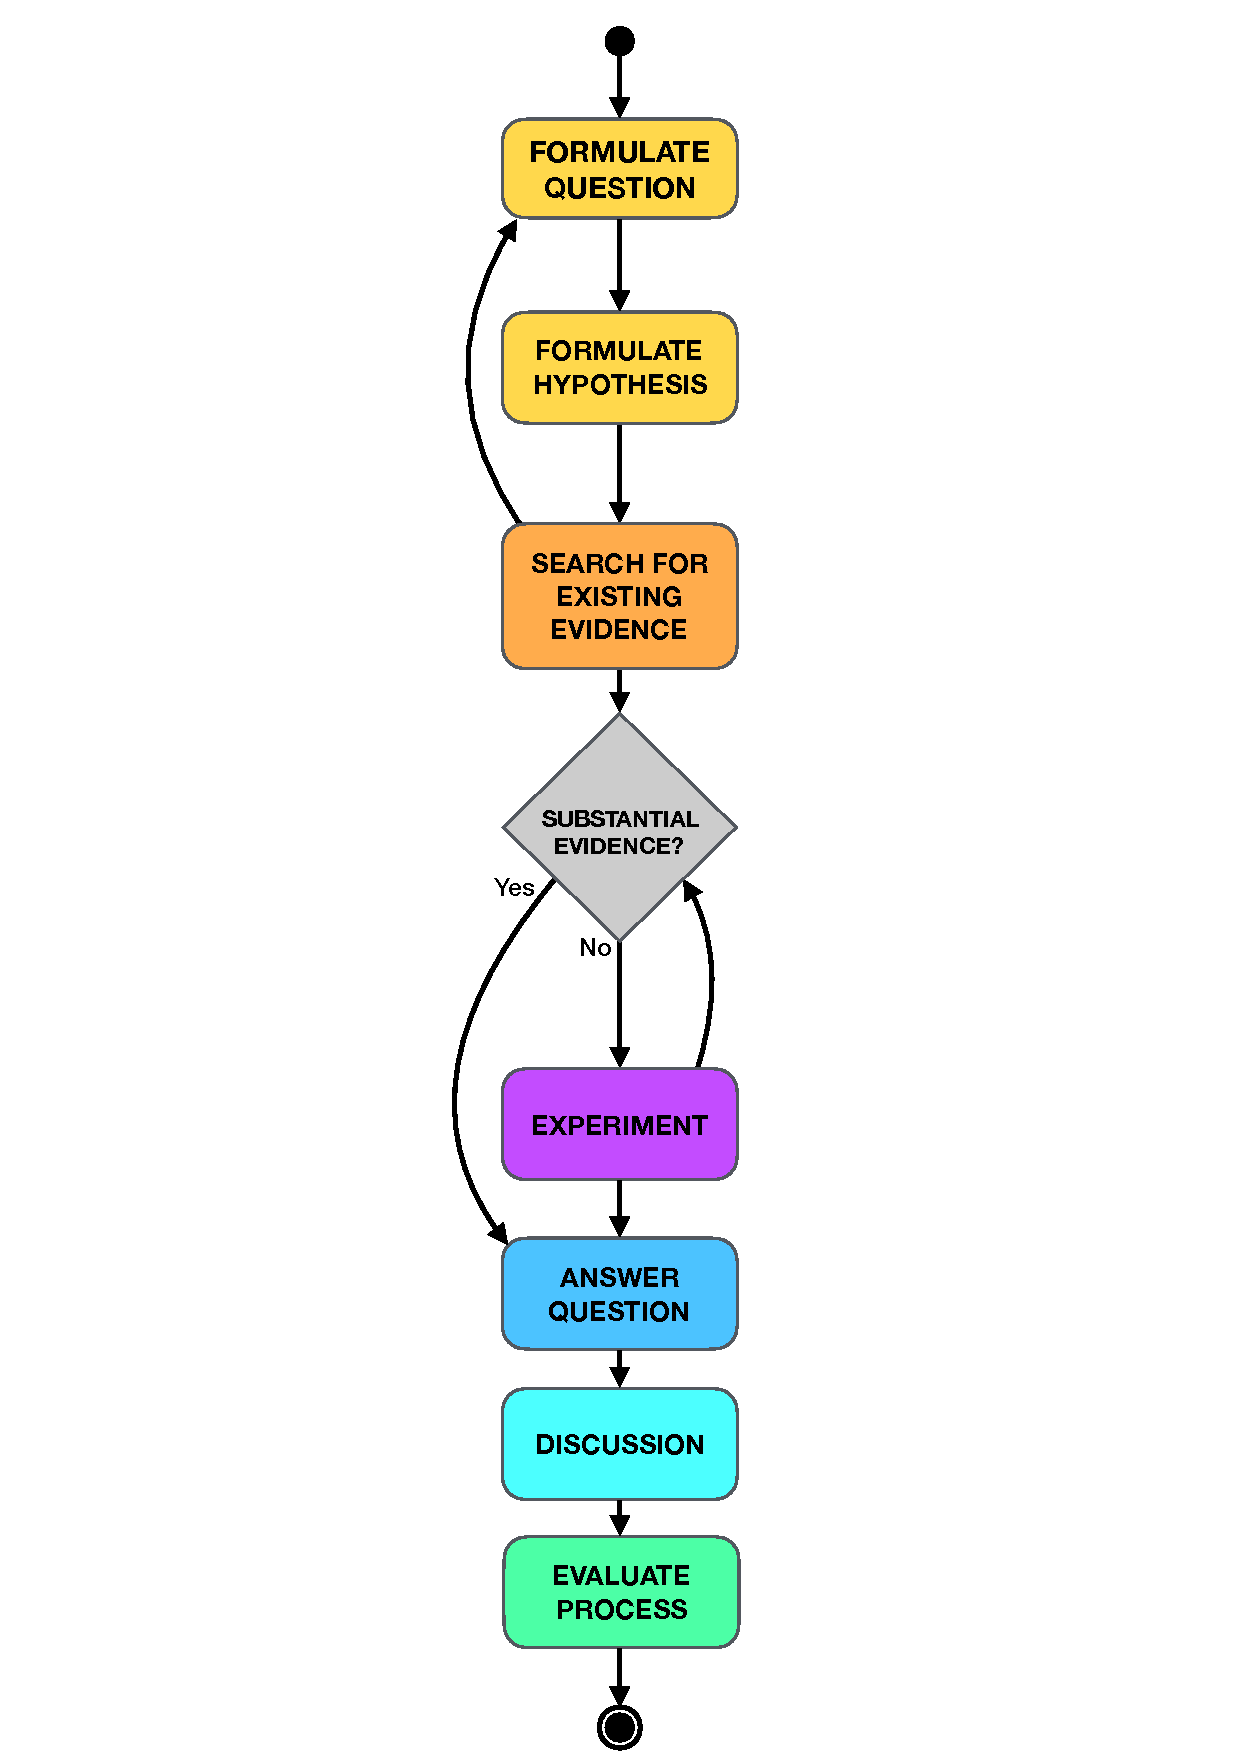
\includegraphics[trim={3cm 0 3cm 0}, height=14.55cm]{figures/workflow_graph.pdf}
	\caption{Workflow Graph}
	\label{fig:workflow_graph}
\end{wrapfigure}


In this section, a document called \emph{Student Process Improvement Document (\checklist{})} is introduced. It is supposed to guide students through scientific working with EBSE in mind.

Rainer \etal found, that \q{[s]tudents varied in their use of the EBSE checklist} \cite{Rainer2006} (see issue \ref{itm:issue5} in table \ref{table:issuesEBSE}). Therefore, an important design criteria for \checklist{} is ease of use through clear and simple instructions. Especially tailored for students with little knowledge about scientific working in general.

The process of \checklist{} contains eight steps:
\begin{enumerate}
\item Formulate question
\item Formulate hypothesis
\item Search for existing evidence
\item Substantial evidence
\item Experiment
\item Answer question
\item Discussion
\item Evaluate process
\end{enumerate}


The whole graph can be seen in figure \ref{fig:workflow_graph}. The actual document can be found in appendix \ref{appendix:checklist}.\\
On the left of the document, a flow chart of the proposed process is depicted. For computer science students this should be a fast way to navigate through and orient themselves in the process. To further assist navigation visually, each process step has been assigned a unique color. This color schemes reoccurs in the tools section of the document as well as in \briefingform.

On the right additional information is given. Each process step in \checklist{} contains a short description, some guidelines, and acceptance criteria. The guidelines contain methods and tools on how to process the current step. The acceptance criteria give students orientation on when a step is completed.
\end{minipage}











\section{Briefing Form}
TODO
	The checklist (TODO name?) is meant to implicitly guide the user's approach to experimenting.
By guiding the user, typical mistakes might be prevented.
To create guidelines that help preventing typical users' mistakes, these mistakes first need to be identified.
In this section, experiences and guidelines found in related work are discussed.
The conclusions are used as basis for design of our guidelines.
The first set of guidelines is based on the report of Rainer et al. \cite{Rainer2006}:

\begin{center}
	\begin{tabular}{ | p{6cm} | p{7cm} |}
	\hline
	\textbf{Observation} & \textbf{Conclusion/Guideline} \\ \hline
	
	\obsrvQuote{Students had problems constructing well-formulated EBSE questions.} (p. 6) 
	& Give examples for good questions to make sure the user understands a good question's scope of 
	information. Also, explicitly list which building blocks should be contained in the question. \\ \hline
	
	\obsrvQuote{Students used limited criteria for identifying the best or better evidence[...]} (p. 6) 
	& Support decision-making to get a decision as unbiased and suited as possible.
	Since a decision's quality is highly dependent on the individual case, we only give a very general hint to
	the user. The idea is to sensitize the user to consciously prevent bias as good as possible. \\ \hline
	
	\obsrvQuote{Students used a very limited number of search terms.} (p. 6) 
	& If users look for something very specific without knowing the technical term, search engines might yield
	better results when used with more detailed search terms.
	Also, synonyms or similar words might widen the search's scope to find more related work.
	Encourage more search terms by providing examples containing enough search terms. \\ \hline
	
	\obsrvQuote{Students provided poor explanation in their reports of how their searches were conducted.}
	(p. 7)
	& TODO \\ \hline
	
	\obsrvQuote{Students varied in their use of the EBSE checklist.} (p. 7)
	& Design the checklist in a way to support the user's workflow instead of hindering it.
	Keep it possibly simple and provide enough examples to make the user never guess an item's 
	meaning. \\ \hline
	
	\obsrvQuote{Some students critically appraise the technologies rather than the publications (evidence) on
	the technologies} (p. 7)
	& TODO Give a hint/indication? \\ \hline
	
	\obsrvQuote{But we also think that the kinds of problems students were tackling [...] are not the kinds of 
	problems researchers commonly investigate.} (p. 8)
	& Scientific and practical evidence can have very different requirements regarding content and other
	aspects such as duration of evaluation. To limit this paper's scope, we focus on scientific evidence. \\ \hline
	\end{tabular}
\end{center}
	\begin{itemize}
	\item in this paper we propose a one page briefing of research study
	\item supports EBSE and searchability of study
	\item similar to SEED but more detailed structure to support searchability even more.
	\item supports researcher in understanding the field of research
	\item supports researcher in understanding the study itself
	\item guides researcher through study design and result documentation process
	\item contains of: research question, hypothesis, experiment/context or deduction, conclusion
	\item experiment contains: independent and dependent variables (control variables), method, results  
\end{itemize}


\fbox{\begin{minipage}{\linewidth}
		{\large\textbf{Question}}\\
		Contains \textbf{\textit{technology}} in a \textbf{\textit{context}} showing an \textbf{\textit{effect}}. TODO Kitchenham Quote (practitioners)?\\
		\exampleQuote{Does pair programming in professional software development teams increases code quality?}
		\\
		\\
		\\
		{\large\textbf{Hypothesis}}\\
		Needs to contain a \textbf{\textit{prediction}} and needs to be \textbf{\textit{testable}}.\\
		\exampleQuote{If you do x, then y will happen}
		\\
		\\
		\\
		{\large\textbf{Experiment}}\\
		\textbf{Context}\\
		\\
		\textbf{Dependent Variables}\\
		Variables that are  \textbf{\textit{measured}} during the study.\\
		\\
		\textbf{Independent Variables}\\
		Variables that are  \textbf{\textit{changed}} during the study.\\
		\\
		\textbf{Method}\\
		Lab-/Field study, number of participants, metrics, ...\\
		\\
		\textbf{Results}\\
		Experiment's outcome\\
		\textbf{No} interpretation or conclusion!\\
		\\
		\\
		\\
		{\large\textbf{Conclusion}}\\
		Interpretation of experiment's results.\\
		Verifying or Falsifying Hypothesis.\\
		Scope of generalization.
\end{minipage}}

% !TEX root = ../../seminar.tex

\section{Discussion}
\label{sec:discussion}

To support students in scientific working, this paper introduced a process along with guiding documents.
The process is mainly based on EBSE.\\
The workflow and documents were not evaluated in this work. Therefore, they need to be tested in future work. This should be done with students in real world scenarios such as bachelor and master theses. Comparing multiple theses is a difficult task. There are many influencing factors and already a certain variance in the quality of theses requiring a lot of subjects. Also finding a suiting metric to classify and compare two theses that might not be particularly similar is not trivial. Whereas asking students in a qualitative study can provide useful insight whether the documents were actually helpful or not.\\
When formatively evaluated, a digitalized version of \briefingform{} should be implemented to allow state of the art data collection and searching. This is a step towards an infrastructure which supports the use of EBSE on a larger scale. That kind of infrastructure might also be of interest for software practitioners and scientists.

\bibliographystyle{splncs03}%
\bibliography{seminar}%

\end{document}
